\section{STM in ABS}
\label{sec:stm_abs}
In this section we give a short overview of how we apply STM in our ABS. In both case-studies we fundamentally follow a time-driven, parallel approach as introduced in Chapter \ref{sub:par_strategy}, where the simulation is advanced by a given $\Delta t$ and in each step all agents are executed. To employ parallelism, each agent runs within its own thread and agents are executed in lock-step, synchronising between each $\Delta t$, which is controlled by the main thread. See Figure \ref{fig:stm_abs_structure} for a visualisation of our concurrent, time-driven lock-step approach.

By running each agent in a thread will guarantee the execution in parallel even if the agent has a monadic context. This is forces us to evaluate each agents monadic context separately instead of running them all in a common context. Note that ultimately we are ending up in the \textit{IO} context because \textit{STM} can be only transacted from within an \textit{IO} context due to non-deterministic side-effects. This is no contradiction to our original claim: yes we are running in IO but not the agent behaviour itself, which is a fundamental difference.

An agent thread will block until the main-thread sends the next $\Delta t$ and runs the \textit{STM} action atomically with the given $\Delta t$. When the \textit{STM} action has been committed, the thread will send the output of the agent action to the main-thread to signal it has finished. The main thread awaits the results of all agents to collect them for output of the current step e.g. visualisation or writing to a file.

As will be described in subsequent sections, central to both case-studies is an environment which is shared between the agents using a \textit{TVar} or \textit{TArray} primitive through which the agents communicate concurrently with each other. To get the environment in each step for visualisation purposes, the main thread can access the \textit{TVar} and \textit{TArray} as well. 

\begin{figure}
	\centering
	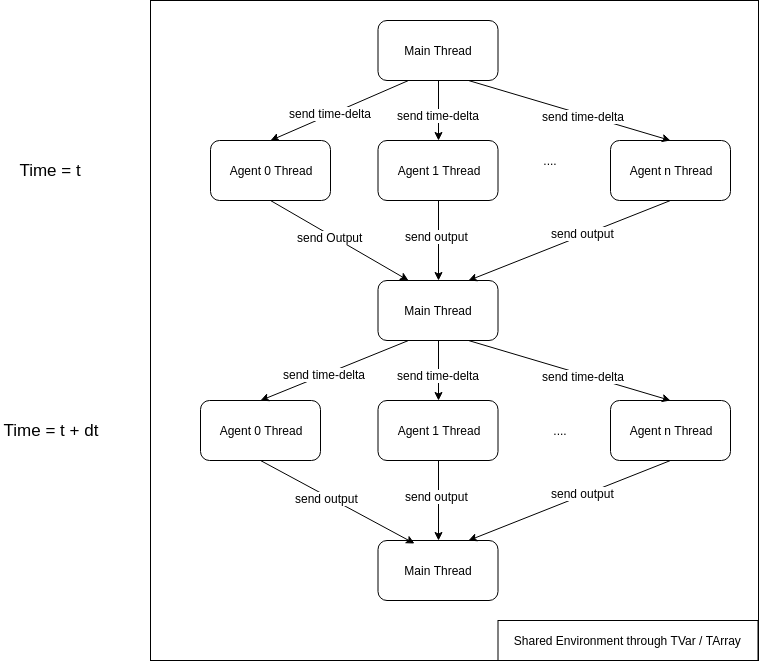
\includegraphics[width=1.0\textwidth, angle=0]{./fig/concurrentabs/stm_abs.png}
	\caption{Diagram of the parallel time-driven lock-step approach.}
	\label{fig:stm_abs_structure}
\end{figure}

\subsection{Adding and running the STM Monad}
We briefly show how to add STM to agents and run them within their own threads. We use the SIR implementation as example - applying it to the Sugarscape implementation works exactly the same way and is left as a trivial exercise to the reader.

The first step is to simply add the \textit{STM} to the existing transformer stack as the \textit{innermost} monad. The reason why we make it the innermost is to guarantee that in case of a retry \textit{all} outer monadic effects are retried as well - if the STM would be placed on a higher stack level, the levels below would not be subject to a retry. For monads like the \textit{ReaderT} this would not matter because they are read-only but for a StateT this fact would matter a lot. Note that STM does not provide a transformer instance, so this is not an option anyway. If STM would provide a transformer then we could make \textit{IO} the innermost monad and do \textit{IO} within STM, which should be prevented under all circumstances because then rolling back a transaction cannot guarantee to undo the effects. To better understand the semantics of retries consider the following example:

\begin{HaskellCode}

\end{HaskellCode}



\begin{HaskellCode}
innerSTMAction :: RandomGen g => StateT SomeState (RandT g STM) SomeResult

let randAction = runStateT innerSTMAction initState
let stmAction  = runRandT randAction (mkStdGen 42)
let ioAction   = atomically stmAction
((someResult, someState), g) <- ioAction
\end{HaskellCode}

In this case the STM is the \textit{innermost} monad thus it will be run last. This means that all the outer monads are subject to re-computation due to retries.

\begin{HaskellCode}
outerSTMAction :: STMT (StateT Environment (Rand g)) SomeResult

let ioAction = runSTMT outerSTMAction
stateAction <- ioAction
let randAction = runStateT stateAction initState
let ((someResult, someState), g) = runRandT randAction (mkStdGen 42)
\end{HaskellCode}

In this case, the STM is the \textit{outermost} monad, thus it will be run first. This means that it will return a StateT computation which will be computed \textit{after} the STM has transacted. The computation construction is subject to the retries but the computation itself won't be repeated in case of retries.

TODO: add STM

\begin{HaskellCode}
agentThread :: RandomGen g 
            => Int
            -> SIRAgent g
            -> g
            -> MVar SIRState
            -> MVar DTime
            -> IO ()
agentThread 0 _ _ _ _ = return () -- all steps computed, terminate thread
agentThread n sf rng retVar dtVar = do
  -- wait for dt to compute current step
  dt <- takeMVar dtVar

  -- compute output of current step
  let sfReader = unMSF sf ()
      sfRand   = runReaderT sfReader dt
      sfSTM    = runRandT sfRand rng
  ((ret, sf'), rng') <- atomically sfSTM -- run the STM action atomically within IO

  -- post result to main thread
  putMVar retVar ret
  
  -- to next step
  agentThread (n - 1) sf' rng retVar dtVar
\end{HaskellCode}

\begin{HaskellCode}
simulationStep :: TVar SIREnv
               -> [MVar DTime]
               -> [MVar SIRState]
               -> DTime
               -> IO SIREnv
simulationStep env dtVars retVars dt = do
  -- tell all threads to continue with the corresponding DTime
  mapM_ (`putMVar` dt) dtVars
  -- wait for results but ignore them, SIREnv contains all states
  mapM_ takeMVar retVars
  -- return state of environment when step has finished
  readTVarIO env
\end{HaskellCode}